%!TEX root = mb.tex

% 2nd fig/1st fig = 1.12 ratio
\begin{figure*}[t!]

\centering
\subfigure[Enterprise to external site communication]{
  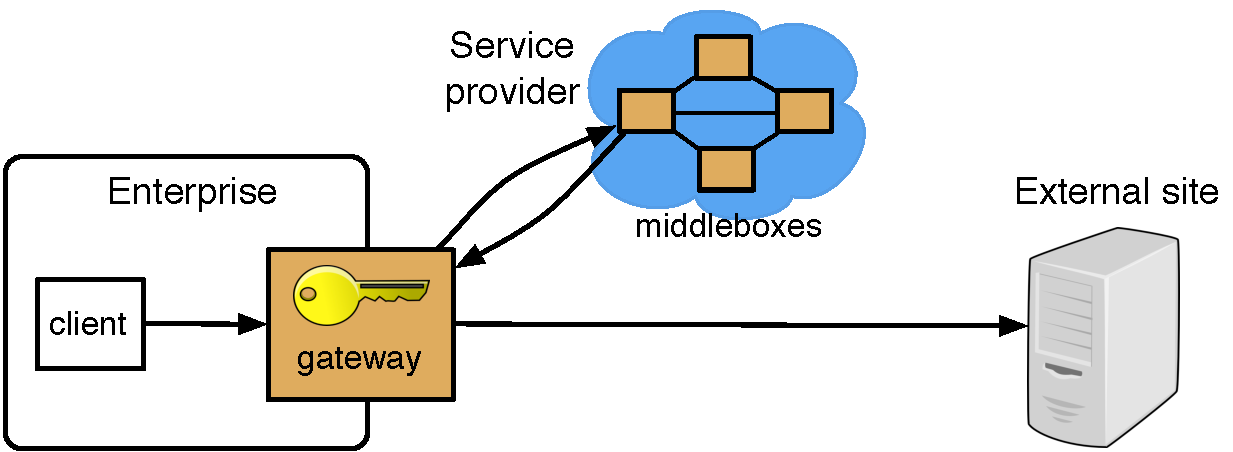
\includegraphics[width=2.8in]{fig/model_1.pdf}
  \label{fig:model1} }
%
\hfill  
\subfigure[Enterprise to enterprise communication]{
   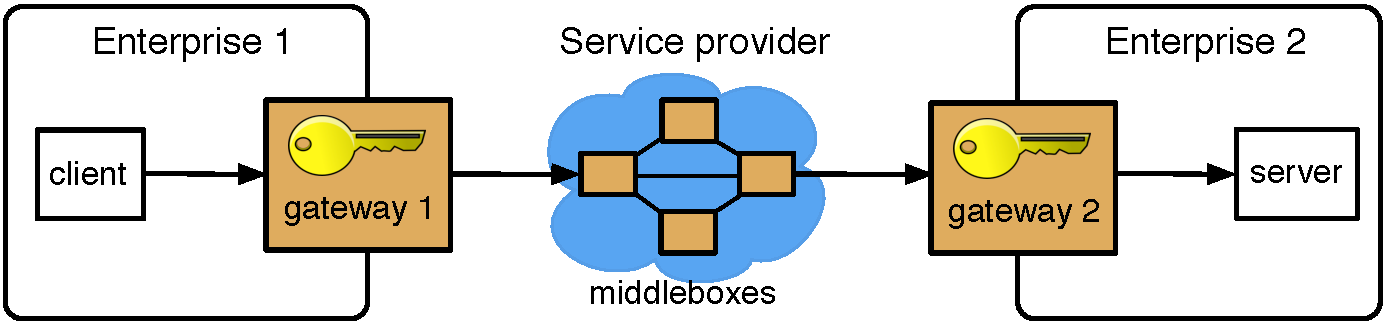
\includegraphics[width=3.2in]{fig/model_2.pdf}
     \label{fig:model2}}
     
     %
\caption{System architecture. APLOMB and NFV system setup with \sys encryption  at the gateway. The arrows indicate traffic from the client to the server; the response traffic follows the reverse direction. \label{fig:sys-overview}}
\end{figure*}
     
\section{Overview}\label{sec:overview}

In this section, we present \sys's architecture, the threat model and applications supported.


% TO CUT REMOVE: just mentino the figures and no need to explain 
\subsection{System Architecture}

\sys uses the same  architecture as APLOMB~\cite{aplomb}, a system which redirects an enterprise's traffic to the cloud for middlebox processing. \sys augments this architecture with confidentiality protection.

%The benefits of outsourcing are to delegate the burden of managing and configuring
%middleboxes (e.g., upgrading, deciding which vendor to use, monitoring), reduce costs of hardware,
%and provide elasticity and fault tolerance; hence \sys should maintain these benefits despite any changes made to to the gateway at the enterprise or middleboxes.

In the APLOMB setup, there are two parties: the enterprise(s) and the service provider (SP).
The enterprise runs a gateway (GW) which sends traffic to a set of middleboxes (MB) running in the cloud; in practice this cloud may be either a public cloud service (such as EC2), or an ISP-supported service running at a Central Office (CO).
%we already said thisThe service provider -- ISP or cloud-based -- runs a set of middleboxes. 

We illustrate the two redirection setups from APLOMB in Fig.~\ref{fig:sys-overview}.  The first setup, in Fig.~\ref{fig:model1},  occurs when the enterprise communicates with an external site: traffic goes to the cloud and back before it is sent out to the Internet. 
It is worth mentioning that APLOMB allows an optimization that saves on bandwidth and latency relative to Fig.~\ref{fig:model1}: the traffic from SP can go directly to the external site and does not have to go back through the gateway. \sys does not allow this optimization fundamentally: the traffic from SP is encrypted and cannot be understood by an external site. 
Nonetheless, as we demonstrate in \S\ref{sec:eval}, for ISP-based deployments this overhead is negligible.
For traffic within the same enterprise, where the key is known by two gateways owned by the same company, we can support the optimization as shown in Fig.~\ref{fig:model2}.

We do not delve further into the details, motivation, and gains of APLOMB's setup, and refer the reader to~\cite{aplomb} for details. 

%\eat{
%\begin{table}
%\centering
%\small
%\hspace{-2pt}
%\begin{tabular}{l|l|p{.45in}|p{.45in}|p{.45in}}
%&{\bf MB}&{\bf TCP/IP Header}&{\bf HTTP Headers}&{\bf Byte Stream}\\
%
%\hline
%
%\parbox[t]{1mm}{\multirow{3}{*}{\rotatebox[origin=c]{90}{Header}}}
%&IP Firewall&Range&-&-\\
%&L4 LB&Range&-&-\\
%&NAT&Exact&-&-\\
%\hline
%
%
%\parbox[t]{1mm}{\multirow{2}{*}{\rotatebox[origin=c]{90}{DPI}}}
%&IPS&Range&Exact&Exact\\
%&Exfiltration&Range&Exact&Exact\\
%\hline
%
%\parbox[t]{1mm}{\multirow{3}{*}{\rotatebox[origin=c]{90}{HTTP}}}
%&Proxy&Exact&Exact&-\\
%&Parent Filter&-&Exact&-\\
%&L7 LB&Exact&Exact&-\\
%\hline
%*&VPN&-&-&-\\
%
%\end{tabular}
%\caption[]{Middleboxes supported by \sys and categorized as Header, DPI, or HTTP middleboxes depending on what fields they access. Middleboxes are also labeled whether they perform `exact match' comparisons against rules, or `range match' comparisons against rules.\label{tbl:mbreqs}} 
%\end{table}
%}

\subsection{Threat Model}
%%%I know this may read superfluous to a security reader but two of the SOSP reviewers asked for this specifically -- why is a passive attacker a reasonable choice? We need this background here.
%Before defining our threat model precisely, we first provide context and background on the concerns clients have about cloud providers today.
  Clients adopt cloud services for decreased cost and ease of management. Providers are known and trusted to provide good service. 
  However, while clients trust cloud providers to perform their services correctly, there is an increasing concern that cloud providers may access or leak confidential data in the process of providing service.
  Reports in the popular press describe companies selling customer data to marketers~\cite{radioshack}, disgruntled employees snooping or exporting data~\cite{att}, and hackers gaining access to data on clouds~\cite{databreach,PrivacyRecords}.
  This type of threat is referred to as an `honest but curious' or `passive'~\cite{goodrich} attacker: a party who is trusted to handle the data and deliver service correctly, but who looks at the data, and steals or exports it.  Hence, \sys aims to stop these attackers.
  Such an attacker differs from the `active' attacker, who manipulates data or deviates from the protocol it is supposed to run~\cite{goodrich}.
%
Hence, we consider that such a passive attacker has gained access 
to {\em all the data at SP}.
This includes any traffic and communication SP receives from the 
gateway, any logged information, cloud state, and so on.  
 
We assume that the gateways are managed by the enterprise and hence trusted; they do not leak information.
%The goal of \sys is to protect the privacy of the traffic against an attacker at the service provider  
%cloud employee, or hacker gaining access to cloud machines). 

%The existence of this gateway is they key difference between BlindBox and \sys and not only changes our trust model, but also allows us to improve performance, privacy, and deployability relative to BlindBox, as we will discuss lated in this paper.

Some middleboxes (such as intrusion or exfiltration detection) have a threat model
of their own about the two endpoints communicating. For example, intrusion detection assumes that 
one of the endpoints could misbehave, but at most one of them misbehaves~\cite{Bro}.  
%(indeed, if both misbehave, they can send attack traffic to each other encrypted with a shared symmetric key and fundamentally
%no one can detect such an attack).  
We preserve these threat models unchanged. These applications rely
on the middlebox to detect attacks in these threat models. Since we assume the middlebox executes
its functions correctly and \sys preserves the functionality of these middleboxes, 
these threat models are irrelevant to the protocols in \sys, and we will not discuss them again. 

\subsection{Encryption Overview}

\begin{figure*}[t!]
\begin{center}
  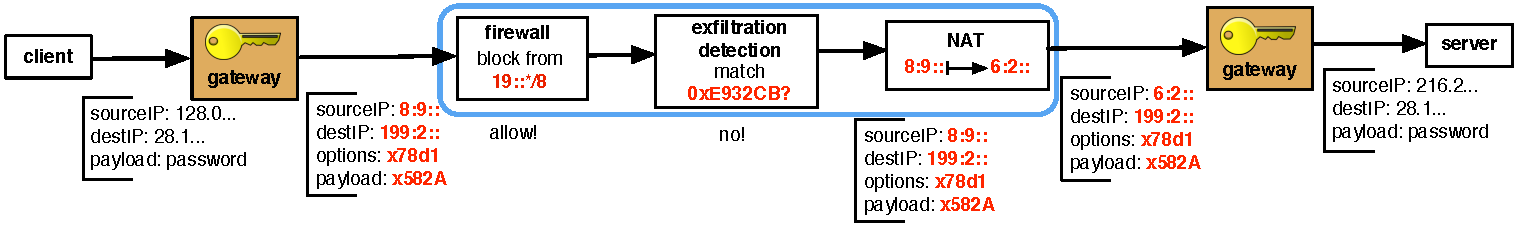
\includegraphics[width=6.7in]{fig/packetpath.pdf}
\caption{Example of packet flow through a few middleboxes. Red in bold indicates encrypted data. \label{fig:packetflow}}
\end{center}
\end{figure*}

To protect privacy, \sys \textit{encrypts all traffic} passing through the service provider (SP).
\sys encrypts the entire packet, including payloads and headers; the enterprise knows the contents of these packets but SP does not. One might ask why do we want to encrypt headers as well. Communication includes endpoints and contents, and both types of information should not be revealed. While contents are carried in the packet payloads, information about endpoints are mostly in the headers. 

\sys also provides the cloud provider with a set of {\it encrypted rules}.
Typically, header policies like firewall rules are generated by a local network administrator. Hence, the gateway knows these rules, and these rules may or may not be hidden from the cloud.
DPI and filtering policies on the other hand may be private to the enterprise (as in exfiltration policies), known by both parties (as in  public blacklists), or known only by the cloud provider (as in  patented malware signatures).
We discuss how rules are encrypted, generated and distributed given these different trust settings in \S\ref{sec:rulenc}.

As in Fig.~\ref{fig:sys-overview}, the gateway has a secret key $k$; in the setup with two gateways, they share
the same secret key. 
At setup time, the gateway generates the set of encrypted rules using $k$ and provides them to SP.
Afterwards, the gateway encrypts all traffic going to the service provider using \sys's encryption schemes.
The middleboxes at SP process  encrypted traffic, comparing the traffic against the encrypted rules. 
After the processing, the middleboxes
will produce encrypted traffic which SP sends back to the gateway. The gateway decrypts the traffic using the key $k$.

Throughout this process, middleboxes at SP handle only encrypted traffic and never access the decryption key. 
On top of \sys's encryption, the gateway can use a secure tunneling protocol, such as SSL or IPSec to secure the communication to SP.




\noindent\textbf{Packet encryption.}
The key idea is to encrypt packets {\it field-by-field}: \eg{}  an encrypted packet will contain a source address that is an encryption of the original packet's source address. We ensure that the encryption has the same size as the original data, and place any additional encrypted information or metadata in the options field of a packet. 

\sys uses three encryption schemes to protect the privacy of each field while allowing comparison against encrypted rules at the cloud: 

\begin{myitemize}
\item Traditional AES: provides strong security and no computational capabilities
\item KeywordMatch:  allows the provider to detect if an encrypted value in the packet is equal to an encrypted rule; does not allow two encrypted values to be compared to each other
\item PrefixMatch: allows the provider to detect whether or not an encrypted value lies in a range of rule values -- e.g. addresses in 128.0.0.0/24 or ports between 80-96.
\end{myitemize}
We discuss these cryptographic algorithms in \S\ref{sec:buildingblocks}.

For example, we encrypt IP addresses using PrefixMatch. This allows, e.g., a firewall to check whether the packet's source belongs to a prefix known to be controlled by a botnet -- but without learning what the actual source IP address is.
We choose which encryption scheme is appropriate for each field based on a high level classification of middlebox capabilities.
Table~\ref{tbl:mbreqs} shows a list of all middleboxes supported by typical outsourcing deployments~\cite{aplomb} and their processing requirements.
We classify these middleboxes as operating only over L3/L4 headers, operating only over L3/L4 headers and HTTP headers, or operating over all data including arbitrary fields in the connection bytestream (DPI).
We revisit them in detail in \S\ref{sec:mbs}.

All encrypted packets are converted to IPv6 because our PrefixMatch scheme requires 128 bits to encode an encrypted IP address  -- and because we expect more and more service providers to be moving to IPv6 by default in the future.
This is a trivial requirement as it is easy to convert from IPv4 to IPv6 (and back) at the gateway~\cite{siit}; clients may continue using IPv4 and the tunnel connecting the gateway to the provider may be either v4 or v6.

{\bf Example.} Fig.~\ref{fig:packetflow} shows the end-to-end flow of a packet through three example middleboxes in the cloud, each middlebox operating over an encrypted field.  
First,  the gateway encrypts the packet as explained above. The packet passes through the firewall which tries to match the encrypted information from the header against its encrypted rule, and decides to allow the packet. Next, the exfiltration device checks for any suspicious (encrypted) strings in data encrypted for DPI and not finding any, it allows the packet to continue to the NAT. The NAT maps the source IP address to a different IP address. Back at the gateway, the gateway decrypts the packet. 

\subsection{Functionality}

Table~\ref{tbl:mbreqs} lists the middleboxes supported by \sys along with the concrete functionality \sys supports.
\sys supports the ``textbook'' functionality of most middleboxes considered for outsourcing in APLOMB~\cite{aplomb}.
  In this paper, we consider the functionality of the middlebox to be the core, reference description\todo{add cite}. We note that there exist versions of these middleboxes with more complex functionality that \sys may not support: we discuss \sys's limitations in \S\ref{s:limitations}.

Nevertheless, \sys covers the ``textbook'' functionality for almost all these middleboxes. Such functionality covers many real use cases; as a demonstration, we show in \S\ref{sec:eval} that \sys supports at least one real usage for each one of the middlebox categories in Table~\ref{tbl:mbreqs}.


% sys supports the textbook functionality of almost all middleboxes considered for outsourcing in aplomb. 
% for each category of middlebox, \sys supports at least one real use case as we show in \s. 


\subsection{Architectural Implications} 
\label{sec:bbarch}
%%%End the discussion wiht BB here.
%%% DO NOT DELETE.

As mentioned, when compared to BlindBox, \sys provides new cryptography and system designs to support  more general middleboxes --  it turns out that, on top of these, the architectural setting of \sys provides additional benefits, which we can now explain.


%new encryption scheme and a new system design that enables a complete set of middleboxes, 
%So far, we have described the overall architecture of \sys without discussing how the encryption or middleboxes themselves are implemented.
%It is worth pausing here to discuss how this architecture itself can improve BlindBox, although it only supports DPI.
%
The first benefit is increased performance. In BlindBox, two arbitrary user endpoints communicate over a modified version of HTTPS. BlindBox requires 97 seconds to perform the initial handshake, which results in the encryption of the rules. 
This exchange must be performed for every new connection in BlindBox because each session is between two new endhosts with a per-connection key.
However, in the \sys context, this exchange can be performed just once at the gateway because the connection between the gateway and the cloud provider is long-lived. Consequently, there is no per-connection overhead. 
%, after which the same encrypted rules can be reused for all clients; this key is safe to re-use because it is private to the gateway.
%Most importantly, this architecture provides practical performance, where the BlindBox context imposed a prohibitive per-connection overhead.


The second benefit is increased deployability. In \sys, the gateway encrypts traffic where in BlindBox the end hosts do. Hence, deployability improves because the end hosts do not need to be modified.

Finally, security improves in the following way.
BlindBox has two security models: a stronger one to detect rules that are `exact match' substrings, and a weaker one to detect rules that are regular expressions. The more rules there are, the higher the per-connection setup cost is. 
Since there is no per-connection overhead  in \sys, we can afford having more rules. 
Hence, we convert many regular expressions to a set of exact-match strings. 
For example /hello[1-3]/ is equivalent to exact matches on "hello1", "hello2", "hello3".
Nonetheless, many regular expressions remain too complex to do so -- if the set of potential exact matches is too large, we leave it as a regular expression.
As we show in \S\ref{sec:eval}, this approach halves the number of rules that require using the weaker security model, enabling more rules in the stronger security model. 

In the rest of the paper, we do not revisit these architectural benefits, but focus  on \sys's new capabilities that allow us to outsource a {\it complete} set of middleboxes.
